%! TEX root = Calculo.tex
\documentclass{../Calculo.tex}


\begin{document}
\section{Bibliografía}
\begin{itemize}
	\item Stewart, J. Cálculo en varias variables.
	\item Apuntes de Pepe Aranda.
	\item Tom M. Apostol, "Calculus".
	\item Tom M. Apostol, Análisis Matemático.
\end{itemize}
\pagebreak
\section{El espacio $\R^{n}$}
\subsection{El conjunto $\R^{n}$}
$\R^{n}$ es el conjunto
\[
		\R^{n} =\{ ( x_1,\dots ,x_{n}) / x_{i} \in \R, 1 \leq i \leq n\}
\]
De momento, este conjunto no tiene ninguna estructura. Para ello, se introduce
la noción de espacio vectorial (EV a partir de ahora).
\begin{itemize}
	\item La suma vectorial:
	\[
		\vec{a} + \vec{b} = (a_{i}+b_{i},\dots a_{n}+b_{n})	
	\]
	\item Producto por escalar:
		\[
			k \vec{a} = (ka_{1},\dots ,ka_{n})
		\]
\end{itemize}
Con estas dos operaciones, $\mathbb{R}^{n}$ es EV, y a sus elementos, los vamos a
llamar vectores, y los denotaremos por $\vec{x}=(x_{1},\dots x_{n})$.\\
Con esta estructura, los elementos de $\mathbb{R}^{n}$ se pueden ordenar, por
ejemplo, en una cuadrícula.
\begin{center}

\tikzset{every picture/.style={line width=0.75pt}} %set default line width to 0.75pt        

\begin{tikzpicture}[x=0.75pt,y=0.75pt,yscale=-1,xscale=1]
%uncomment if require: \path (0,300); %set diagram left start at 0, and has height of 300

%Straight Lines [id:da3051942297151431] 
\draw    (231,181) -- (345,181) ;
\draw [shift={(347,181)}, rotate = 180] [color={rgb, 255:red, 0; green, 0; blue, 0 }  ][line width=0.75]    (10.93,-3.29) .. controls (6.95,-1.4) and (3.31,-0.3) .. (0,0) .. controls (3.31,0.3) and (6.95,1.4) .. (10.93,3.29)   ;
%Straight Lines [id:da9246749315532883] 
\draw    (231,181) -- (307.83,74.62) ;
\draw [shift={(309,73)}, rotate = 125.84] [color={rgb, 255:red, 0; green, 0; blue, 0 }  ][line width=0.75]    (10.93,-3.29) .. controls (6.95,-1.4) and (3.31,-0.3) .. (0,0) .. controls (3.31,0.3) and (6.95,1.4) .. (10.93,3.29)   ;




\end{tikzpicture}	
\end{center}

\subsection{$\mathbb{R}^{n}$ como espacio afín}
Nos será útil para definir direcciones desde cualquier punto de $\mathbb{R}^{n}$.
La estructura afín en $\mathbb{R}^{n}$ se define por la aplicación
\[
	\varphi: \mathbb{R}^{n} \times \mathbb{R}^{n} \mapsto \mathbb{R}^{n}
\]
\[
	(\vec{u}, \vec{v}) \mapsto \varphi(\vec{u}, \vec{v})
\]
donde $\varphi(\vec{u}, \vec{v})$ se representará como un vector cuyo punto
de aplicación está en el extremo de $\vec{u}$ y el extremo, el de $\varphi(
\vec{u}, \vec{v})$ en el extremo de $\vec{v}$. Es fácil comprobar que
\[
	\varphi(\vec{u},\vec{v}) = \vec{v} - \vec{u}
\]
En este contexto es conveniente llamar puntos a los vectores con punto de
aplicación en el $\vec{0}$ y vectores a los vectores cuyo punto de aplicación
es arbitratio. Los puntos también los denotaremos mediante letras mayúsculas,
y los vectores con letras minúsculas.
\begin{center}
	

\tikzset{every picture/.style={line width=0.75pt}} %set default line width to 0.75pt        

\begin{tikzpicture}[x=0.75pt,y=0.75pt,yscale=-1,xscale=1]
%uncomment if require: \path (0,300); %set diagram left start at 0, and has height of 300

%Straight Lines [id:da9620131632250988] 
\draw    (251,201) -- (367,201) ;
%Straight Lines [id:da5426532654970737] 
\draw    (251,201) -- (329,93) ;
%Straight Lines [id:da23784315263106715] 
\draw [color={rgb, 255:red, 0; green, 0; blue, 0 }  ,draw opacity=1 ]   (367,201) -- (329.66,94.89) ;
\draw [shift={(329,93)}, rotate = 70.62] [color={rgb, 255:red, 0; green, 0; blue, 0 }  ,draw opacity=1 ][line width=0.75]    (10.93,-3.29) .. controls (6.95,-1.4) and (3.31,-0.3) .. (0,0) .. controls (3.31,0.3) and (6.95,1.4) .. (10.93,3.29)   ;

% Text Node
\draw (387,203.4) node [anchor=north west][inner sep=0.75pt]    {$P$};
% Text Node
\draw (294,58.4) node [anchor=north west][inner sep=0.75pt]    {$Q$};
% Text Node
\draw (357,110.4) node [anchor=north west][inner sep=0.75pt]    {$\varphi ( P,Q) =\overrightarrow{PQ}$};


\end{tikzpicture}
\end{center}
A recordar que punto - punto define un vector, y que punto + vector = punto.
Con esto ya podemos definir direcciones.
\subsection{$\mathbb{R}^{n}$ como espacio métrico}
Para medir longitudes, ángulos y distancias introduciremos en $\mathbb{R}^{n}$
el \textbf{producto escalar}.
\begin{defin}
	El producto escalar entre dos vectores $\vec{u}$ y $\vec{v}$ se define como
	\[
		\cdot : \mathbb{R}^{n} \times  \mathbb{R}^{n} \mapsto \mathbb{R}
	\]
	\begin{equation}
		\begin{split}
			\vec{u} \cdot  \vec{v} = \sum_{i=1}^{n} u_{i}v_{i}
		\end{split}
	\end{equation}
	El producto escalar tiene las propiedades siguientes:
	\begin{itemize}
		\item $\vec{u} \cdot  \vec{v} = \vec{v} \cdot \vec{u}$
		\item $\vec{u} \cdot (\vec{v}+\lambda\vec{w})= 
			\vec{u} \cdot \vec{v} + \lambda \vec{u} \cdot \vec{w}$
		\item $\vec{u} \cdot \vec{u} \geq 0 \implies \vec{u} \cdot \vec{u}=0
			\iff \vec{u} = \vec{0}$ 
	\end{itemize}
\end{defin}
Debido a la propiedad 3, podemos definir la longitud (o norma) de un vector como
\begin{defin}
	La longitud o norma de un vector se define como:
	\begin{equation}
		\begin{split}
			|\vec{u}| = \sqrt{\vec{u} \cdot \vec{u}} = \sqrt{\sum_{i=1}^{n}
			u_{i}^{2}}
		\end{split}
	\end{equation}
	Las propiedades son que:
	\begin{itemize}
		\item $|\vec{v}| = 0 \iff \vec{v} = 0$
		\item $|\lambda \vec{u}| = |\lambda| |\vec{u}|$
		\item Desigualdad de Cauchy-Schwarz:
			\[
				|\vec{u} \cdot \vec{v}|\leq |\vec{u}||\vec{v}|
			\]
		\begin{proof}[Demostración]
			Observemos que si uno de los vectores es el vector nulo, entonces
			la desigualdad se satisface por igualdad, o también si ambos vectores
			son proporcionales entre sí. Supongamos entonces que $u$ y $v$ son LI.
			Eso significa que la ecuación $u=\lambda v$ no tiene solución.
			\[
				u - \lambda v = \vec{0}
			\]
			\[
				(u-\lambda v)(u-\lambda v) = 0
			\]
			\[
				u \cdot u - 2xu\cdot v+x^{2} v\cdot v=0
			\]
			Recordando la definición de norma queda
			\[
				x^{2}|v|^{2}-2xu\cdot v + |u|^{2}=0
			\]
			Ahora tenemos una ecuación de segundo grado en $x$. Como no puede
			tener solución, $b^{2}-4ac < 0$.
			\[
				(2u\cdot v)^{2} -4|v|^{2}|u|^{2} < 0
			\]
			\[
				2|u\cdot v| < 2|v||u|
			\]
			\[
				|u\cdot v|<|v||u|
			\]
			Como deben cumplirse ambas
			\begin{equation}
				\begin{split}
					|u\cdot v| \leq |v||u|
				\end{split}
			\end{equation}
		\end{proof}
		\item Desigualdad triangular
			\[
				|\vec{u}+\vec{v}| \leq |\vec{u}|+|\vec{v}|
			\]
		\begin{proof}[Demostración]
			Partimos de $u+v$
			\[
				(u+v)\cdot (u+v)=|u|^{2}+2u\cdot v+|v|^{2} = |u+v|^{2} \geq 0
			\]
			Por Cauchy-Schwarz, $u\cdot v\leq|u\cdot v| \leq |u|\cdot |v|$
			\[
				|u+v|^{2} \leq |u|^{2} + |v|^{2} + 2|u||v|
			\]
			\[
				|u+v|^{2} \leq (|u|+|v|)^{2}
			\]
			\[
				|u+v| \leq |u|+|v|
			\]
		\end{proof}
	\end{itemize}
\end{defin}
De especial importancia son los vectores con norma $1$, denominados como
\textbf{vectores unitarios}.
\begin{defin}
	Definimos como vectores unitarios a esos vectores $\vec{v}$ que cumplen que
	\begin{equation}
		\begin{split}
			|\vec{v}| = 1
		\end{split}
	\end{equation}
\end{defin}
Mediante la desigualdad de Cauchy-Schwarz, podemos obtener un método para medir
ángulos. Observemos que de C-S se deduce 
\begin{equation}
	\begin{split}
		||u||v|| \leq u\cdot v \leq |u||v|
	\end{split}
\end{equation}
Si ninguno de los vectores es el nulo, podemos dividir entre las normas
\begin{equation}
	\begin{split}
		-1\leq\frac{u\cdot v}{|u||v|} \leq 1
	\end{split}
\end{equation}
Entonces, como está acotada en $[-1,1]$, podemos definir el ángulo $\alpha$ entre
$u$ y $v$ como
\begin{defin}
	El ángulo $\alpha$ entre $u$ y $v$ como el ángulo que satisface
	\begin{equation}
		\begin{split}
			\cos \alpha = \frac{u\cdot v}{|u||v|}
		\end{split}
	\end{equation}
	donde $\alpha \in [0,\pi]$. Es de relevancia que $\alpha$ siempre se mide como
	el ángulo "interior" o el más pequeño.
	\begin{center}
		

\tikzset{every picture/.style={line width=0.75pt}} %set default line width to 0.75pt        

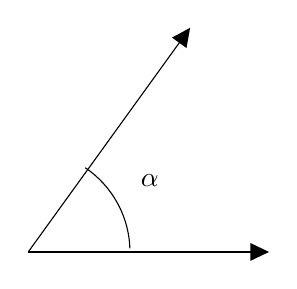
\begin{tikzpicture}[x=0.75pt,y=0.75pt,yscale=-1,xscale=1]
%uncomment if require: \path (0,300); %set diagram left start at 0, and has height of 300

%Straight Lines [id:da4204681338418119] 
\draw    (271,221) -- (384,221) ;
\draw [shift={(387,221)}, rotate = 180] [fill={rgb, 255:red, 0; green, 0; blue, 0 }  ][line width=0.08]  [draw opacity=0] (8.93,-4.29) -- (0,0) -- (8.93,4.29) -- cycle    ;
%Straight Lines [id:da9882209281394811] 
\draw    (271,221) -- (347.24,115.43) ;
\draw [shift={(349,113)}, rotate = 125.84] [fill={rgb, 255:red, 0; green, 0; blue, 0 }  ][line width=0.08]  [draw opacity=0] (8.93,-4.29) -- (0,0) -- (8.93,4.29) -- cycle    ;
%Shape: Arc [id:dp7205301342242372] 
\draw  [draw opacity=0] (298.46,180.41) .. controls (311.02,188.93) and (319.42,203.13) .. (319.97,219.32) -- (271,221) -- cycle ; \draw   (298.46,180.41) .. controls (311.02,188.93) and (319.42,203.13) .. (319.97,219.32) ;  

% Text Node
\draw (324,182.4) node [anchor=north west][inner sep=0.75pt]    {$\alpha $};


\end{tikzpicture}
	\end{center}
	Si $\alpha = \frac{\pi}{2} \implies u\cdot v = 0 \implies$ $u$ y $v$ son
	\textbf{ortogonales}.\\
	Aunque el ángulo entre $\vec{0}$ y otro vector cualquiera no está definido,
	sin embargo, se suele decir que $\vec{0}$ es ortogonal a todos los vectores de
	$\mathbb{R}^{n}$ 
\end{defin}
Ahora en $\mathbb{R}^{2}$ ya podemos dibujarlos "correctamente". Ahora falta
definir distancias entre puntos de $\mathbb{R}^{n}$.
\begin{defin}
	Definimos la distancia entre dos puntos $P$ y $Q$ como   
	\begin{equation}
		\begin{split}
			d(P,Q) = |\vv{PQ}| = |Q-P|
		\end{split}
	\end{equation}
\end{defin}
\subsection{Rectas e hiperplanos en $\mathbb{R}^{n}$}
Una recta en $\mathbb{R}^{n}$ que pasa por un punto $P$ y tiene la dirección
$\vv{v} \in \mathbb{R}^{n}$ se define como los puntos $X$ que satisfacen
\begin{equation}
	\begin{split}
		X = P+t\vv{v}
	\end{split}
\end{equation}
\begin{center}
	

\tikzset{every picture/.style={line width=0.75pt}} %set default line width to 0.75pt        

\begin{tikzpicture}[x=0.75pt,y=0.75pt,yscale=-1,xscale=1]
%uncomment if require: \path (0,300); %set diagram left start at 0, and has height of 300

%Straight Lines [id:da2796590956331695] 
\draw    (260,155) -- (401.11,106.65) ;
\draw [shift={(403,106)}, rotate = 161.09] [color={rgb, 255:red, 0; green, 0; blue, 0 }  ][line width=0.75]    (10.93,-3.29) .. controls (6.95,-1.4) and (3.31,-0.3) .. (0,0) .. controls (3.31,0.3) and (6.95,1.4) .. (10.93,3.29)   ;
%Straight Lines [id:da5188733313816549] 
\draw  [dash pattern={on 4.5pt off 4.5pt}]  (122,203) -- (514.53,68.5) ;

% Text Node
\draw (230,139.4) node [anchor=north west][inner sep=0.75pt]    {$P$};
% Text Node
\draw (337,66.4) node [anchor=north west][inner sep=0.75pt]    {$\vec{v}$};


\end{tikzpicture}
\end{center}
La recta está descrita por un solo parámetro libre, por lo que es un objeto de
dimensión $1$. Si $v_{j}\neq 0$ con $j \in \{ 1,\dots ,n \}$  podemos eliminar $t$
\begin{equation}
	\begin{split}
		t = \frac{x_{j}-p_{j}}{v_{j}}
	\end{split}
\end{equation}
Y entonces
\begin{equation}
	\begin{split}
		x_{i} = p_{i} +\frac{x_{j}-p_{j}}{v_{j}}v_{i} ~/~ i \neq j
	\end{split}
\end{equation}
Por tanto, la recta está definida por $n-1$ ecuaciones. Por tanto, la recta
es un objeto de codimensión $n-1$. 
\end{document}
